\chapter{Introduction to the constructive gravity programme}\label{chapter_introduction}

\section{The r\^ole of gravity in physics}
As the title suggests, this thesis is primarily concerned with \emph{gravity}. In the ensemble of physical theories, gravity plays a special r\^ole. It serves a different purpose than the theories we will call \emph{matter theories}. The latter are subject to direct observations: photons---quanta of the electomagnetic field---hit the observers retina, allowing her to make inferences about the source of the particles. Charged fermions---again quanta of a corresponding matter field---induce signals in a semiconductor detector. Specific signatures in the signals may be associated with certain events that contributed to the production of the incident fermions, such that the statistics of these observations is able to falsify hypotheses about the underlying mechanisms.

How does gravity fit into this picture? The revolution of a binary star about its centre of mass, commonly known to be caused by gravity, is not observed directly. Neither are its gravitational spin-up and eventual merger. Rather, the stars emit photons that are picked up by the astronomer, who concludes details about the trajectories. When the LIGO and Virgo Collaborations announced the first observation of gravitational waves \cite{ligo}, the ground-breaking detection was earth-bound, but in a certain sense not \emph{direct}: it amounts to the analysis of interference patterns from photons that bounced off of mirrors at the end of the detector arms. General relativity predicts that these arms should expand and contract under the influence of incident gravitational waves. Eventually, the signature in the interference pattern was found to match the predictions for a binary black hole merger.

\begin{figure}
  \begin{center}
    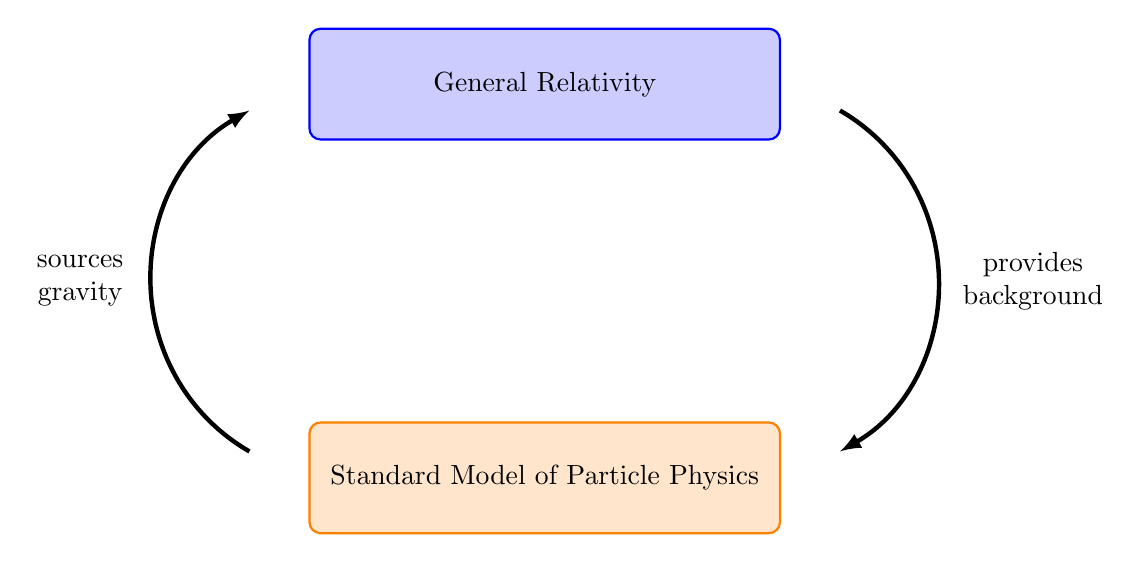
\begin{tikzpicture}[%
      auto,
      block1/.style={rectangle,thick,draw=blue,fill=blue!20,align=center,rounded corners,minimum width=17em,minimum height=4em},
      block2/.style={rectangle,thick,draw=orange,fill=orange!20,align=center,rounded corners,minimum width=17em,minimum height=4em},
      pics/carc/.style args={#1:#2:#3}{code={\draw[pic actions] (#1:#3) arc(#1:#2:#3);}}
      ]
      \draw (0,2.5) node[block1] (G) {General Relativity};
      \draw (0,-2.5) node[block2] (S) {Standard Model of Particle Physics};
      \draw (-2.5,0) pic[latex-,ultra thick]{carc=120:240:2.5};
      \draw (2.5,0) pic[latex-,ultra thick]{carc=-60:60:2.5};
      \draw (-5.9,0) node[align=center] {sources\\gravity};
      \draw (6.2,0) node[align=center] {provides\\background};
    \end{tikzpicture}
  \end{center}
  \caption{Interplay of the standard model theories and general relativity. Matter content sources the gravitational field equations. The gravitational field, in turn, provides the background on which matter fields propagate. Together, this yields a highly accurate fundamental description of the universe.}
  \label{figure_smpp_gr}
\end{figure}

From this point of view, gravity sets the stage for the propagation of matter fields. This is witnessed by the dynamics for matter fields, one example of which is the electromagnetic potential in Maxwell electrodynamics. Its field equations are derived from the action functional
\begin{equation*}
  S_\text{Maxwell}\lbrack A\rbrack = \int\mathrm d^4x \sqrt{-g} g^{ac} g^{bd} F_{ab} F_{cd},
\end{equation*}
which depends on the potential $A$ via the field strength tensor $F = \mathrm dA$. Maxwell's theory of the electromagnetic field has been a huge success as it is the foundation of many applications throughout science. The quantum field theories for the electromagnetic field and similar gauge theories, together with the fermonic sector, form the standard model of particle physics (SMPP), which is widely regarded as the most precisely tested physical theory\footnote{For example, the magnetic moment of the electron has been measured as $g/2 = 1.001\,159\,652\,180\,73(28)$. \cite{http://dx.doi.org/10.1103/PhysRevA.83.052122} Its value as proposed by quantum electrodynamics has been calculated as $g/2 = 1.001\,159\,652\,182\,03(73)$ \cite{https://doi.org/10.1103/PhysRevD.96.019901}. Both the experimentally measured value and the value calculated from quantum electrodynamics agree to more than 12 significant figures.}. Still, these matter theories presuppose knowledge of the spacetime metric $g$ which enters the action for the electromagnetic field above and contributes to other theories of the SMPP in a similar way. Consequently, the SMPP alone lacks \emph{predictivity}: collecting initial data of all physical fields is not enough for the physicist in order to determine the fields in the future, since the metric tensor has to be specified externally. 

One of the many great contributions by Einstein was the prescription of field equations that govern the dynamics of the metric tensor. \cite{einstein_gr} This theory is called \emph{general relativity} and may be derived from the Einstein-Hilbert action functional
\begin{equation*}
  S_\text{Einstein-Hilbert}\lbrack g\rbrack = \int\mathrm \mathrm d^4x \sqrt{-g} R.
\end{equation*}
Einstein's theory provides the missing link between matter and gravity, completing the SMPP to the joint model of SMPP and general relativity sketched in Fig.~\ref{figure_smpp_gr}, which is now predictive. It has also been verified numerous times, both via astronomical observations and \emph{in terra}\footnote{earthbound} experiments, albeit to a lesser degree of certainty\footnote{Only four significant figures of the gravitational constant are known. \cite{https://doi.org/10.1103/FRevModPhys.88.035009} Measurements with higher precision yield conflicting results. \cite{https://doi.org/10.1103/RevModPhys.84.1527}}.

Of course, the division of physical theories into matter theories and gravity is only a \emph{metaphysical} notion. Both make testable predictions about the outcome of experiments; both have been shown to accurately describe reality in a variety of circumstances. But exactly in this metaphysical idea lies the mindset of \emph{constructive gravity}, which seeks to address the search for other (more?) complete pictures of matter and gravity.

\section{Modified gravity from refined matter theories}
Under certain assumptions, Einstein's general relativity is the unique theory that completes the SMPP to a predictive theory of matter and gravity.\cite{lovelock,hkt,deser} The only two unknown parameters that need to be fixed are Newton's gravitational constant and the cosmological constant. This remarkable finding constrains the search for modified theories of gravity: if the mentioned assumptions are taken for granted, the standard model of particle physics can only be completed by general relativity. It is, however, well established that the joint theory of the SMPP and Einstein gravity cannot be universal, due to several inconsistencies.

One example are extreme circumstances, such as the beginning of the universe or the presence of black holes, where the whole formalism breaks down \cite{}. This is one of the justifications for the efforts of finding a quantum theory of gravity.

Even in more benign situations, the observations do not always coincide with the predictions from the SMPP and general relativity. The observed rotation curves of galaxies, for example, do not match the expectations calculated from the visible matter distributions. Starting from a certain minimum distance from the galaxy centre, stars and other matter content rotate with higher velocities than expected. \cite{} This discrepancy generally increases with the radius. \cite{} All proposed solutions \cite{} that may cure this inconsistency have one thing in common---they modify or extend the currently accepted theories of matter and gravity.

There are more observations \cite{} that demonstrate the need for modifications. However such adjustments play out, they are constrained by the uniqueness of Einstein's general relativity in one of the following ways:
\begin{enumerate}
  \item Additional or modified matter fields that make use of the same metric tensor $g$ as the existing matter theories will still couple to general relativity.
  \item Additional or modified matter fields that couple to new geometry---e.g.~a second metric tensor or a tensor of higher rank---render general relativity as theory for a single metric tensor meaningless. A completely new description of gravity is needed, \emph{which may be subject to similar uniqueness theorems}.
  \item Modifications to general realativity itself are incompatible with the uniqueness theorem. This means that either the assumptions from which uniqueness follows must be dropped or that the matter theories have to be modified accordingly---if at all possible.
\end{enumerate}
All three approaches are pursued, as they should be for a systematic search of modified theories. Constructive gravity, the subject of this thesis, is a framework for the structured treatment of approach number two. In most regards, its assumptions are very conservative, as it tries to deviate only ever so slightly from the established models. For example, where standard general relativity is restricted to field equations of second derivative order, constructive gravity keeps this restriction. This is not because other efforts are not deemed worthwile---they certainly are, but different approaches towards modified gravity research should be explored \emph{ceteris paribus}, only making one change at a time. The focus of constructive gravity lies on novel matter theories coupling to nonmetric geometries and the corresponding gravitational implications \emph{within the existing meta-theory of classical physics}. Most importantly, because the framework is kept so close to the standard models, a similar uniqueness theorem can be derived for nonmetric geometries. It will not be as strong as for the SMPP and general relativity, but nevertheless provide a useful parameterization of modified theories of gravity that fall into the second category.

As far as the framework is concerned, any matter theory that satisfies certain formal requirements (e.g.~has field equations of second derivative order) is fair game. The relevance of constructive gravity, however, crucially depends on the kind of matter theory that is proposed. A complete overhaul of physics is generally not desired---the existing models work very well in certain sectors. Any new theory must reproduce this phenomenology in order to be epistemically significant. For this reason, constructive gravity is considered as a tool that guides the derivation of modified gravity from \emph{refined} matter theories.

\section{Canonical and covariant approaches to constructive gravity}
\begin{figure}
  \begin{center}
    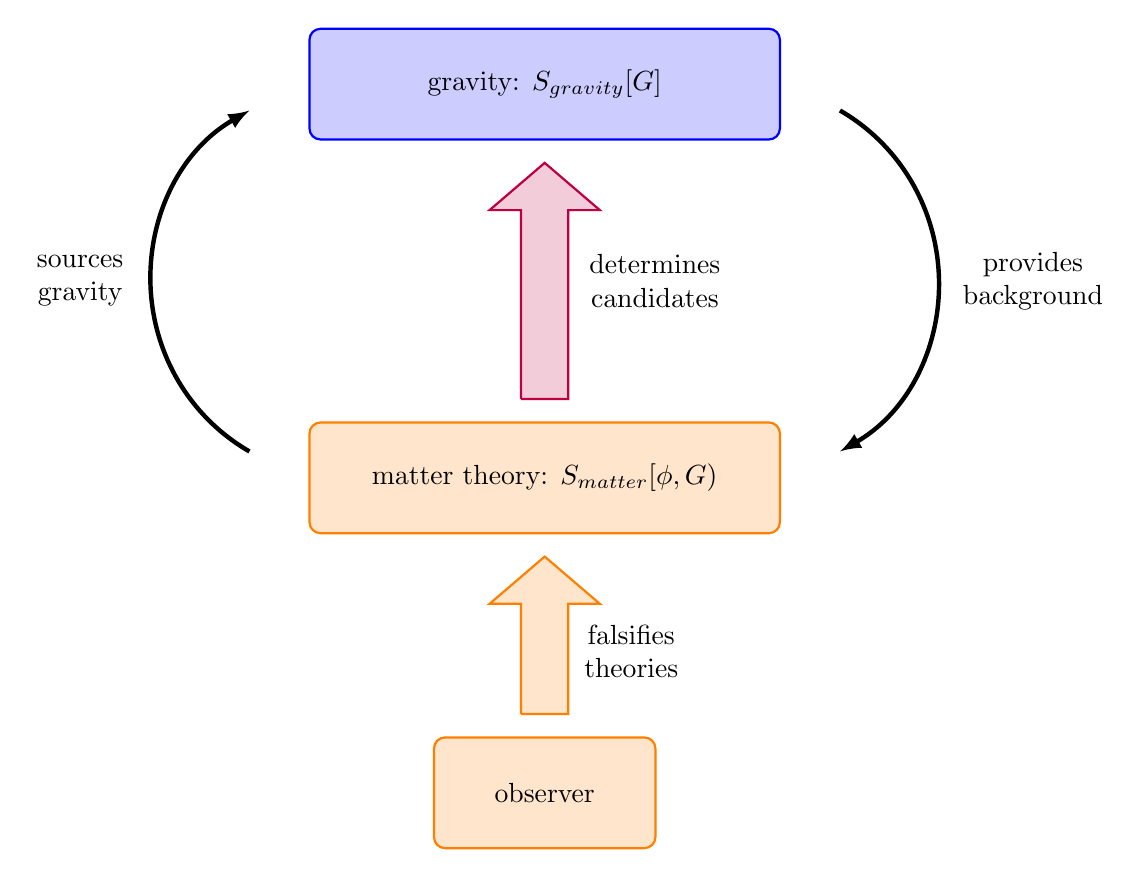
\begin{tikzpicture}[%
      auto,
      block1/.style={rectangle,thick,draw=blue,fill=blue!20,align=center,rounded corners,minimum width=17em,minimum height=4em},
      block2/.style={rectangle,thick,draw=orange,fill=orange!20,align=center,rounded corners,minimum width=17em,minimum height=4em},
      pics/carc/.style args={#1:#2:#3}{code={\draw[pic actions] (#1:#3) arc(#1:#2:#3);}}
      ]
      \draw (0,2.5) node[block1,align=center] (G) {gravity: $S_\text{gravity}\lbrack G\rbrack$};
      \draw (0,-2.5) node[block2,align=center] (S) {matter theory: $S_\text{matter}\lbrack\phi,G)$};
      \draw (-2.5,0) pic[latex-,ultra thick]{carc=120:240:2.5};
      \draw (2.5,0) pic[latex-,ultra thick]{carc=-60:60:2.5};
      \draw (-5.9,0) node[align=center] {sources\\gravity};
      \draw (6.2,0) node[align=center] {provides\\background};
      \draw [thick,draw=purple,fill=purple!20] (-0.3,-1.5) -- (-0.3,0.9) -- (-0.7,0.9) -- (0,1.5) -- (0.7,0.9) -- (0.3,0.9) -- (0.3,-1.5) -- (-0.3,-1.5);
      \draw (1.4,0) node[align=center] {determines\\candidates};
      \draw (0,-6.5) node[block2,align=center,minimum width=8em] (O) {observer};
      \draw [thick,draw=orange,fill=orange!20] (-0.3,-5.5) -- (-0.3,-4.1) -- (-0.7,-4.1) -- (0,-3.5) -- (0.7,-4.1) -- (0.3,-4.1) -- (0.3,-5.5) -- (-0.3,-5.5);
      \draw (1.1,-4.7) node[align=center] {falsifies\\theories};
    \end{tikzpicture}
  \end{center}
  \caption{Rationale of constructive gravity. The matter theory $S_\text{matter}$, which couples the matter field $\phi$ to some geometry $G$, determines the structure of the gravitational theory $S_\text{gravity}$. In general, this theory will not be unique but parameterized by a set of constants or functions, which results in multiple candidates. Via the interdependence of matter and gravity, each candidate yields phenomenology that can be used by the observer for tests of the theory.}
  \label{figure_matter_gravity}
\end{figure}
The rationale of constructive gravity is pictured in Fig.~\ref{figure_matter_gravity}. A matter theory, prescribed by the action $S_\text{matter}\lbrack\phi,G)$ serves as input. The round bracket next to the geometry $G$ indicates that the action functional depends on $G$ only locally, i.e.~not via a derivative, while the matter fields $\phi$ enter with derivatives, typically of first order.

After successful application of constructive gravity, the corresponding gravity action $S_\text{gravity}\lbrack G\rbrack$ that closes the matter theory to a predictive theory of matter \emph{and} gravity is obtained. Staying very close to the established formalism of the SMPP and general relativity, this action is assumed to be of second derivative order in the geometry $G$, with derived field equations also of second derivative order. In general, the gravity action is not unique, it depends on unknown parameters or functions.

This completed theory can now be used for the bread and butter business of theoretical physics: making predictions about the outcome of measurements. Comparisions with experimentally obtained data will restrict the parameter ranges or---if the measurements are incompatible for any parameters---outright falsify the set of theories.

The essence of constructive gravity is the derivation of the gravity action from the matter action, i.e.~the step
\begin{equation*}
  S_\text{matter}\lbrack\phi,G) \Rightarrow S_\text{gravity}\lbrack G\rbrack.
\end{equation*}
Effectively, this amounts to a generalization of the uniqueness theorems for general relativity, which can be interpreted as derivations of Einstein gravity from Maxwell electrodynamics (or, more generally, the SMPP).

\emph{Canonical} constructive gravity (also called \emph{canonical gravitational closure}) \cite{} is the first approach that follows this pattern and is based on the work of Hojman, Kucha\v{r}, and Teitelboim (HKT) \cite{https://doi.org/10.1016/0003-4916(76)90112-3}. HKT showed that the ADM formulation\footnote{The ADM formulation \cite{adm} is a canonical (i.e.~Hamiltonian) formulation of general relativity. Due to the diffeomorphism invariance of general relativity, the canonical formulation is a constrained Hamiltonian system.} of general relativity is the unique representation of the so-called hpyersurface deformation algebra\footnote{A hypersurface is an embedding of a three-dimensional manifold in the four-dimensional spacetime manifold. Different embeddings are related via deformations. The actions of such deformations on hypersurface functionals form an algebra, the \emph{hypersurface deformation algebra}. See \cite{https://doi.org/10.1016/0003-4916(76)90112-3}.}. The canonical approach to constructive gravity considers the hypersurface deformation algebra in a frame that corresponds to an observer subject to matter dynamics. Crucial for the definition of observer frames is the \emph{principal polynomial} of the matter field equations, which captures the causality of the evolution of matter fields (see Sect.~\ref{sect_causal_compatibility}). It then imposes this algebra onto the constraint algebra of the canonical formulation of the unknown gravitational theory. This amounts to a system of functional differential equations, which are subsequently transformed into an infinite system of linear partial differential equations. These equations are called the \emph{construction equations} or \emph{closure equations}. Any solution to this system is a candidate Lagrangian for gravity.

In line with the already known results, general relativity has been shown to be the unique solution to the closure equations of canonical constructive gravity if the procedure is applied to Maxwell's electrodynamics as underlying matter theory. \cite{} However, based on previous work concerning matter theories that couple to arbitrary tensorial geometries \cite{sergio_phd}, the framework has been developed to be applicable to a wide range of matter theories. Two important examples of modified gravitational theories have been derived in linearized form. The first is \emph{area metric gravity} \cite{linear_area_paper}, which completes a birefringent generalization of Maxwell's electrodynamics\footnote{See Sect.~\ref{section_gled}.}. Although only valid for weak gravitational fields, this theory based on a physically well motivated refinement of Maxwell's electrodynamics offers interesting phenomenology when studying quantum electrodynamics \cite{roberto_paper}, gravitational lensing \cite{frederic_marcus_paper}, or gravitational waves \cite{nils_alex_mg15}. \emph{Bimetric gravity} \cite{bimetric_paper}, the completion of a theory with two Klein-Gordon fields coupling to two different metric tensors\footnote{See Sect.~\ref{section_bimetric}.}, is a second example. Another interesting sector of solutions is the cosmological sector, which has also been studied in the past \cite{max_phd(paper)}.

\emph{Covariant} constructive gravity\footnote{First proposed in Ref.~\cite{ccg_paper}.} is a complementary approach. More in the tradition of Lovelock's proof \cite{lovelock} for the uniqueness of the Einstein-Hilbert Lagrangian, it derives the gravitational theory that completes a given matter theory by imposing two conditions directly on the spacetime formulation of gravity---hence the attribute ``covariant''. The two conditions will be called the \emph{axioms} of covariant constructive gravity. Informally, they may be formulated as:
\begin{enumerate}
  \item The dynamical laws that govern the gravitational field are generally covariant, i.e.~are independent of the choice of a coordinate system.
  \item The causality of the gravitational field equations is compatible with the causality of the matter field equations. In particular, a consistent co-evolution of all physical fields is guaranteed.
\end{enumerate}
The motivation for these axioms is twofold. First, they once again enforce the principle that any modified theory of gravity should be close, formally, to general relativity---which implements general covariance and has the same causality as the SMPP. This suggests that also modified theories of gravity should be independent of any coordinate choice and at least be \emph{compatible} with the matter causality.

On the other hand, the approach should complement the canonical framework. General covariance in the spacetime formulation is the equivalent for the conditions placed on the constraint algebra in the canonical formulation. As the second axiom, causal compatibility has been chosen because canonical constructive gravity \emph{claims} to achieve something similar: The observer frame is constructed using matter causality, which is why the hypersurface deformation algebra expressed in this frame contains terms related to matter causality. These terms carry over to the gravitational constraint algebra via the canonical construction procedure. This is often interpreted as the gravitational theory inheriting the causality of the matter theory. But there is little reason to believe so---the fact that the gravitational constraint algebra shares these terms with the hypersurface deformation algebra just means that both are expressed using the same frame. Whether this frame bears any significance for the gravitational theory is an unrelated question. In Ref.~\ref{tobi_msc}, it has been found\footnote{As a preliminary result, for theories of first derivative order.} that the canonical constraint algebra of \emph{any} diffeomorphism invariant theory implements the hypersurface deformation algebra, supporting the suspicion that causality may be unrelated. Even though matching causalities are not enforced by the canonical approach, it is still a sensible requirement for a theory of gravity that closes matter theories, so it is explicitly included as second axiom.

\section{Outline}

This thesis is dedicated to the development of the covariant approach. It aims to provide a complete picture of the current state of research, from the foundations to the construction procedure to testable predictions for an exemplary theory. At the end, every part of Fig.~\ref{figure_matter_gravity} will have been addressed.

After this chapter has introduced the rationale of covariant constructive gravity, Chap.~\ref{chapter_axioms} will be concerned with the mathematical foundations. We will walk through Lagrangian field theory in the jet bundle formulation, which allows a precise definition of the first axiom as equivariance condition for the Lagrangian with respect to spacetime diffeomorphisms. This condition is locally equivalent to a system of first-order, linear partial differential equations, the \emph{equivariance equations}. For the derivation, we will make a detour to the global version of the Lagrangian variation problem, which comes with the definition of the so-called \emph{Cartan form}. The Cartan form allows a quite elegant presentation of Noether's first and second theorem---especially the second theorem will prove to be useful later on. Afterwards, we introduce the notions necessary for a formulation of the second axiom. Causal compatibility will be phrased as conditions on certain geometric constructs that arise from the causality of the field equations.

In chapter \ref{chapter_construction_algorithm}, we turn to the implementation of the axioms. While deriving the mathematical formalism, we already laid out most of the implementation details, so it suffices to give a short summary. This will be in the form of a \emph{construction algorithm}. We then consider three examples of matter theories and discuss how the construction algorithm could be applied. The first example will be Maxwell's electrodynamics, for which we recover general relativity as the unique solution. The other two examples, a birefringent generalization of Maxwell's electrodynamics and a bimetric Klein-Gordon theory, have no known generic solution, but we can nevertheless derive some interesting results.




